\section{Extraction of the limit on the cross-section}
\label{sec:limitExtraction}
% ---- ---- ---- ---- ---- ---- ---- ---- ---- ---- ---- ---- ---- ---- ---- ---- ---- ---- ---- ---- ---- ---- ----

One strength of this analysis, with data-driven estimations of the QCD
and $W+$jets backgrounds (using sidebands and $\alpha$), is that we
can treat the full mass range, 170-600 GeV, by the same methods.  We
use the ``Higgs Combination'' package \cite{cite:combine} for setting
exclusion limits. This package is a RooStats\cite{cite:roostats}-based
statistical analysis toolset recommended by the CMS Higgs PAG.  Inputs
to the limit setter are binned graphs and histograms for data,
background and signal Monte Carlo.

The Higgs mass points are, nominally: 170, 180, 190, 200, 250, 300,
350, 400, 450, 500, 550 and 600~GeV. However, given the availability
of 8~TeV samples as of this writing, we produce a limit from a
restricted set of mass points: 180, 200, 300, 400, 450, 500, 550, 600~GeV.
Standard Model Higgs cross sections are described in
Sec.~\ref{sec:MCexpectations}. In addition, because of the lack of
availability of VBF samples, we scale the glu-glu fusion production
samples by the combined cross-sections for glu-glu and vector boson
fusion, as listed in Table~\ref{tab:modxsec}.

\begin{table}[htb]
 \begin{center}
   \begin{tabular}{c|c|c|l}
     \hline
      $m_{H}$ &  $\sigma$(ggF) (pb) & $\sigma$(ggF+VBF) (pb)  \\
      \hline
      180 & 8.874 &  9.856   \\
      200 & 7.127 &  7.9711  \\
      300 & 3.606 &  4.0468  \\
      400 & 2.924 &  3.1783  \\
      450 & 2.003 &  2.2032  \\
      500 & 1.283 &  1.43910 \\
      550 & 0.8141 & 0.93640 \\
      600 & 0.5230 & 0.61988 \\
     \hline
   \end{tabular}
 \end{center}
 \caption{Modified cross-sections used to compensate for VBF contribution
   to the signal.\label{tab:modxsec}}
\end{table}

To set limits we use the full shape information of the $m_{\ell\nu
jj}$ distribution.  The four-body mass window is set roughly by the
position and width of the signal distributions for the different Higgs
mass points. All of the distributions are segregated by lepton flavor
and whether they meet the 2-jet or 3-jet requirements, which represent
independent channel inputs to the limit setter.

The systematics described in Section~\ref{sec:systematics} are treated
as follows when being input to the limit setter:
\begin{itemize}
\item The main background systematics are total background shape
uncertainty and total background normalization uncertainty. 
% The
% 1-sigma up- and down-fluctuated background shape inputs to the limit
% setter are shown in Appendix~\ref{app:limitShapes}, along with the
% nominal shapes.  
Both shape and normalization uncertainties are
treated as uncorrelated across all channels, since they are derived
from fits performed on independent sample sets.
\item JES, MET uncertainty, and pileup are considered negligible for
signal and are otherwise subsumed in the normalization/shape
uncertainties for background, so they are omitted from the limit setter
inputs.
\item Uncertainties on the signal deriving from lepton reconstruction
and selection as well as trigger efficiency are treated as 100\%
correlated across the same-flavor lepton channels, but uncorrelated
between electron and muon channels.
\item Uncertainties on the signal deriving from parton distribution
functions (Table~\ref{tab:signalPDF}), luminosity, and theoretical
cross-section uncertainty are treated as 100\% correlated across all
channels. Since the PDF and cross-section uncertainties for the gluon
fusion process are uniformly worse than those for the vector boson
fusion process, the uncertainties for the former are taken as
applicable to the summed signal yields.
\item Uncertainties on the signal deriving from the final selection
efficiency are treated as uncorrelated across different channels, but as
correlated between quark-quark and glu-glu signal processes for the same
channel.
\end{itemize}

The limit setter is then set to utilize
the ``asymptotic CL$_{s}$''
\cite{cite:asympcls1,cite:asympcls2} method. 
%The final exclusion limit will be calculated with 
%the ``HybridNew CL$_{s}$'' technique.
The resulting median
expected limit with 1- and 2-sigma error bands are plotted.
The limit plots for all four channels combined (electron 2-jets, 
electron 3-jets, muon 2-jets, and muon 3-jets) are shown in
Fig.~\ref{fig:limitsetup:combinedlimit}. 
The background uncertainty is the limiting factor in this analysis.
%%%%%%%%%%%%%%%%%%%%
\begin{figure}[htb] 
  \begin{center}
    \subfigure[]{
      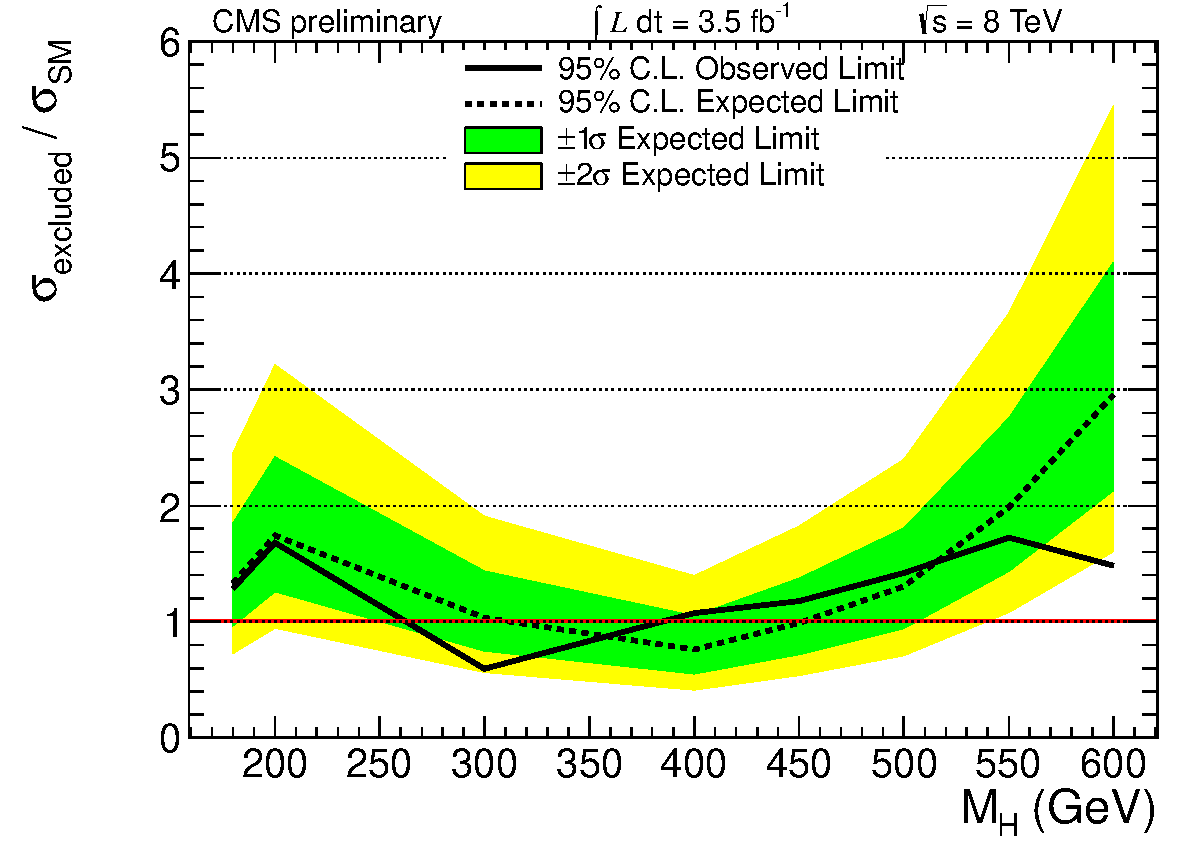
\includegraphics[width=0.48\textwidth]{plots/2012_LIMITS/limit_4chan_fullsyst_asymp.pdf}
%       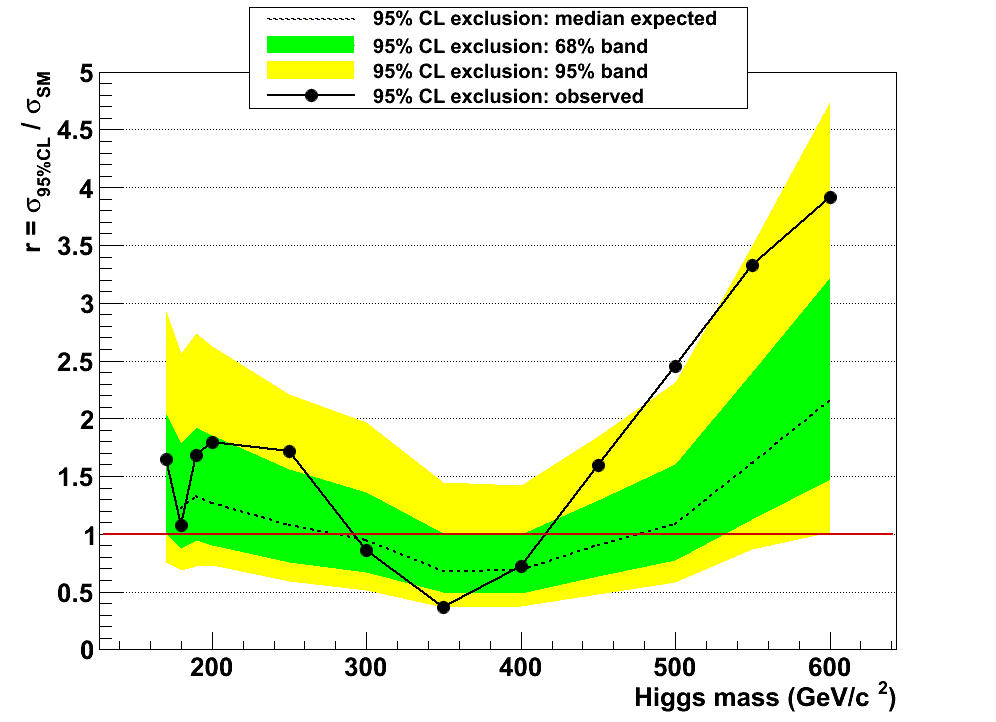
\includegraphics[width=0.6\linewidth]{plots/2012_LIMITS/fullCLs_limits.png}
    }
    \subfigure[]{
      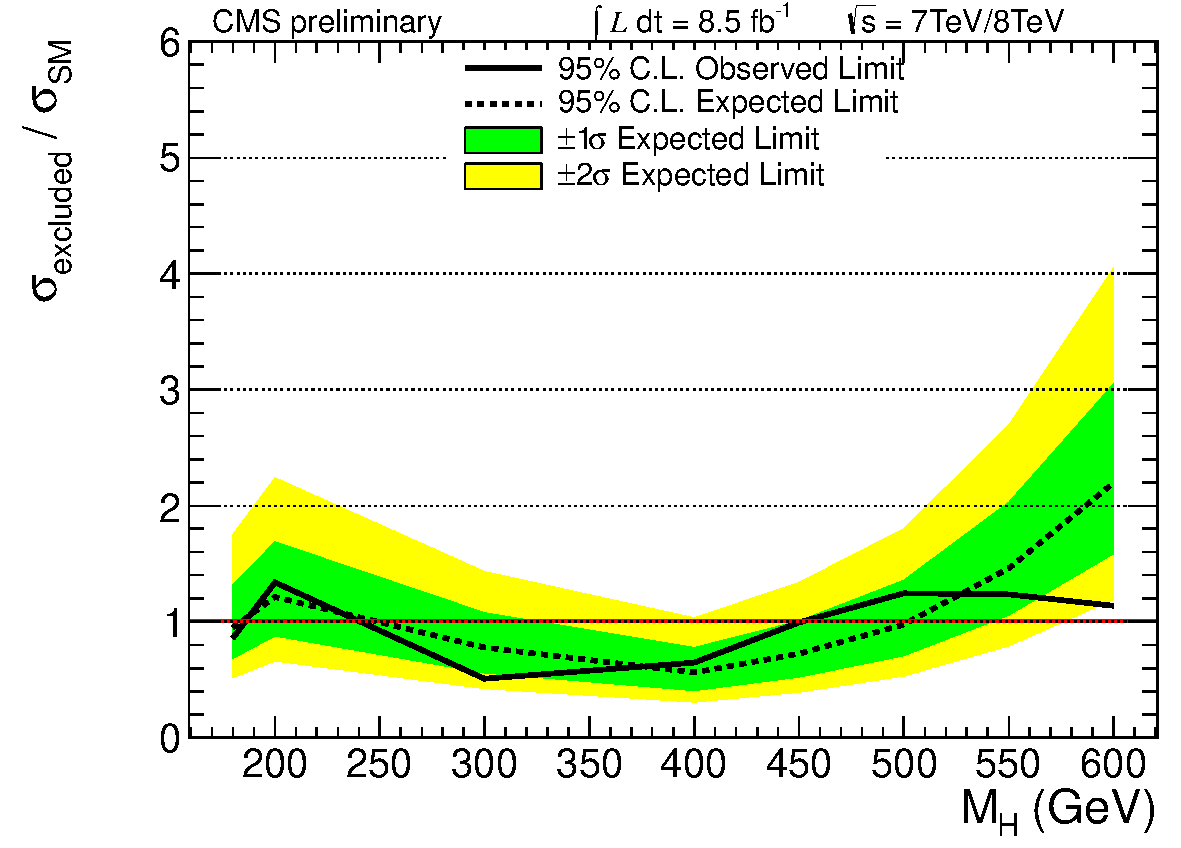
\includegraphics[width=0.48\textwidth]{plots/2012_LIMITS/limit_7and8tevcombined.pdf}
    }
    \caption{The combined Higgs exclusion limit from all four channels
      after including all systematic uncertainties  (a) from 8~TeV data and (b) for 7 and 8~TeV data combined.}
    \label{fig:limitsetup:combinedlimit}
  \end{center}
\end{figure}
%%%%%%%%%%%%%%%%%%%%%%%%%%%%%%%%%%%%%%%%
%%%%%%%%%%%%%%%%%%%%%%%%%%%%%%%%%%%%%%%%
%%%%%%%%%%%%%%%%%%%%%%%%%%%%%%%%%%%%%%%%

Using all four channels of 8~TeV data combined, we exclude the Standard Model 
Higgs boson in the mass range 260--390~GeV, to a confidence level
of 95\%.  When combined with 7~TeV data, the exclusion range expands to 240-450~GeV.
